\section{Testing}

During the course of our project, we conducted various types of testing to ensure the quality and functionality of our application. These tests included unit testing, manual testing by users and customers in the production environment, and more specialized tests for different aspects of the project.

\subsection{Ingestion Performance Tests}

We developed a test infrastructure for the back-end pipeline, focusing on the performance of data ingestion. While we recognized the need to handle large amounts of data in the pipeline, we faced the challenge of mocking this data and incorporating it into our tests. Due to these constraints, we prioritized other aspects of the project and implemented only limited tests for the ingestion performance.

\subsection{User Acceptance Tests}

We collaborated closely with the client throughout the project to meet their requirements and gather valuable feedback. By demonstrating our progress at various stages, we obtained actionable insights that allowed us to refine and enhance the project. This iterative approach ensured that our application met the needs and expectations of its users.

\subsection{UI Tests}

To maintain the quality and functionality of the user interface, we conducted both unit and integration tests for the various components. We utilized Cypress, a JavaScript-based tool using DOM manipulation for automated web tests, to simulate user interactions and assess the performance of our UI components. Currently, we have approximately 30 tests covering essential front-end features such as site navigation, query results, and interactive table functionalities like sorting and filtering. The Cypress testing dashboard can be seen in \autoref{fig:ui-tests}.

\begin{figure}[htp]
    \centering
    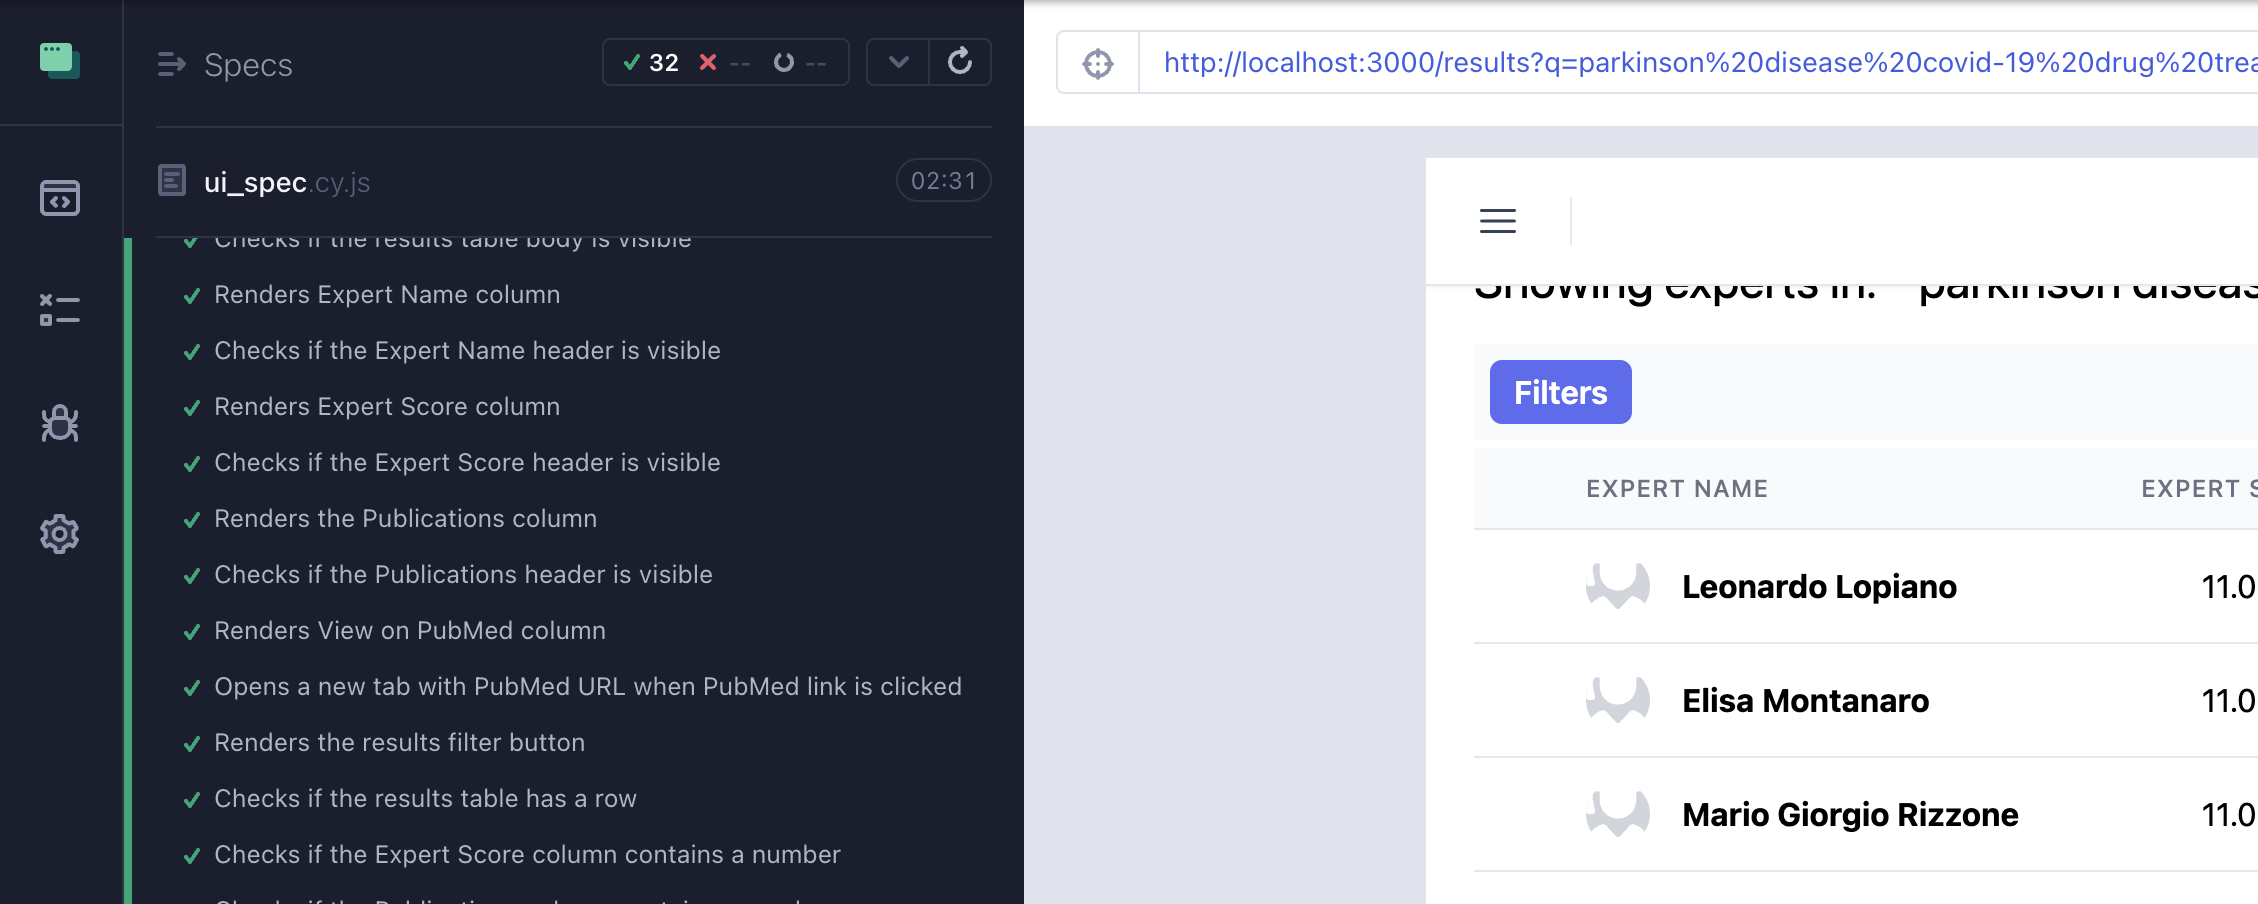
\includegraphics[width=\textwidth]{Images/ui-tests.png}
    \caption[UI Test Results in Cypress Dashboard]{\textbf{A view of the Cypress dashboard showing UI test results:} The Cypress dashboard displays the UI spec testing file, showing 32 passing tests related to user interface functionality. }
    \label{fig:ui-tests}
\end{figure}

\subsection{API Tests}

We employed Postman for API testing in order to validate the requests and responses of our Next.js app's API endpoints. Postman's Runner feature allowed us to simulate front-end application behavior by executing a series of requests concurrently. Currently, we have three endpoints being tested with approximately 20 separate tests in the production environment, all passing successfully, as seen in \autoref{fig:api-tests}.

\begin{figure}[htp!]
    \centering
    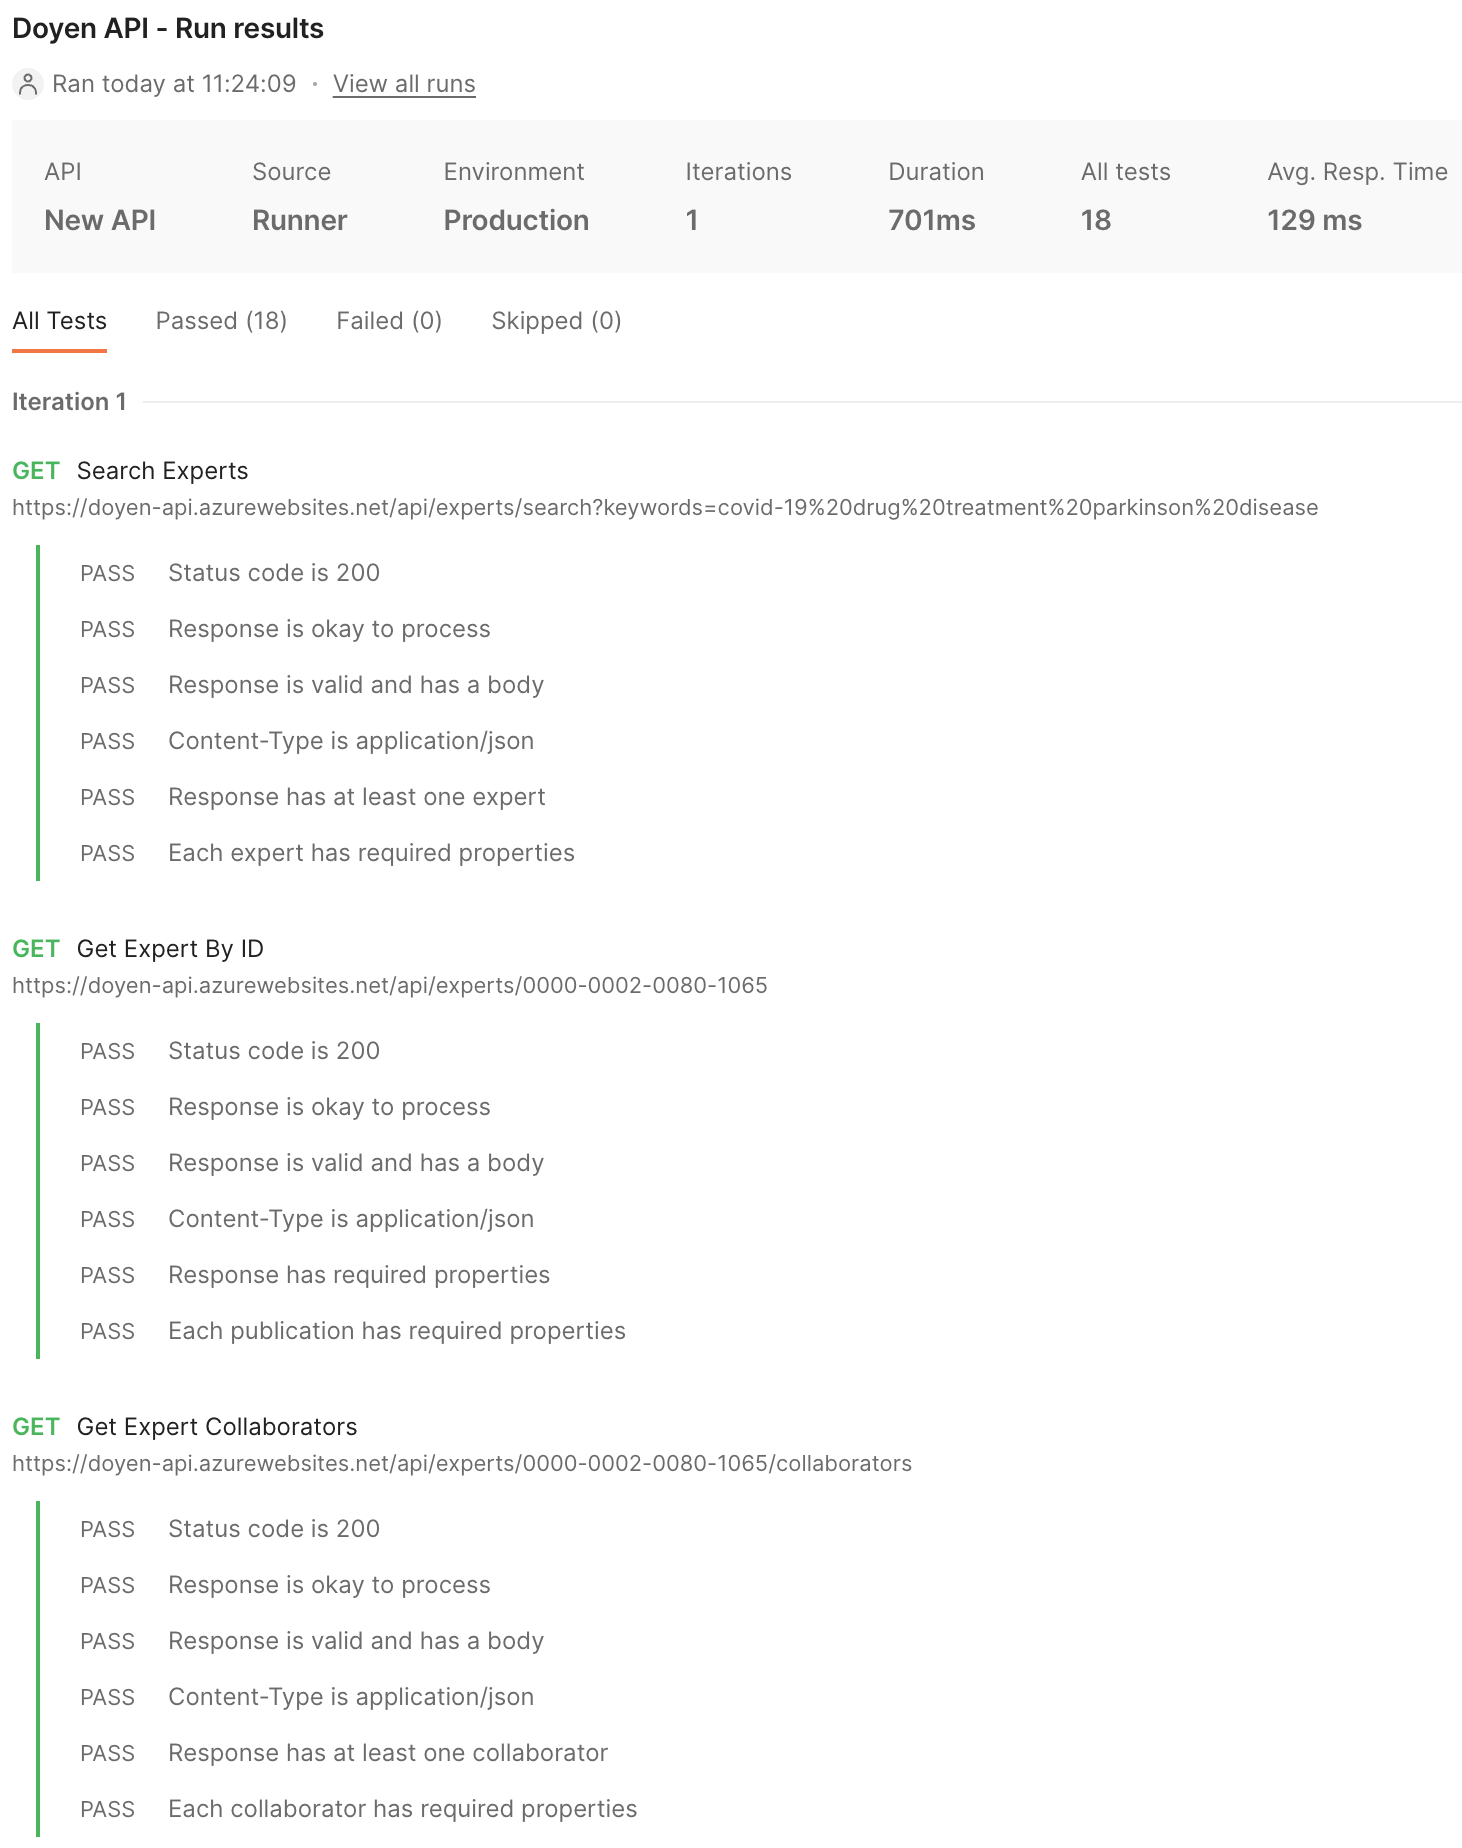
\includegraphics[width=\textwidth]{Images/api-tests.png}
    \caption[API Test Results in Postman Dashboard]{\textbf{A view of the Postman dashboard showing API test results:} The Postman dashboard displays the Doyen API run results, showing 18 passing tests across the three Doyen API endpoints. }
    \label{fig:api-tests}
\end{figure}

In conclusion, by incorporating these various testing methods, we sought to ensure the robustness and reliability of our application while continuously refining its features based on user feedback and requirements. The testing process played a crucial role in the overall success of our project, helping us identify and address potential issues before they could negatively impact the end-user experience.